\subsection{单轨道解的三场分布}
本节对定理 \ref{thm:direct-HMB} 的单轨道三场解作数值计算. 图中使用规范变换前的场 $\widetilde q,\widetilde p,\eta$, 它们由 \eqref{eq:original-fields} 恢复. 取参数
\begin{equation}\label{eq:numerical-parameters}
q_0=1,\qquad a=2,\qquad\eta_0=0.6,\qquad
\alpha=1,\qquad\beta=0.1,\qquad b=1.5,
\end{equation}
范数常数由式 \eqref{eq:onec} 给定, 场值由四维留数系统及无穷远、共振点的重构公式计算. 图 \ref{fig:one} 展示光场的局域振荡及同一区域内的极化和粒子数反转.

\paragraph{先把所有固定参数逐项代入.}
由 $b>q_0$ 的条件, 本例 $1.5>1$ 合法. 原文在式 \eqref{eq:imaginarypoint} 定义的三个量分别为
\begin{align*}
\kappa&=\sqrt{b^2-q_0^2}=\sqrt{1.5^2-1^2}
=\sqrt{2.25-1}=\dfrac{\sqrt{5}}{2},\\
 W&=b+\kappa=\dfrac{3}{2}+\dfrac{\sqrt{5}}{2}
=\dfrac{3+\sqrt{5}}{2},\\
h_0&=\dfrac{q_0}{W}=\dfrac{2}{3+\sqrt{5}}
=\dfrac{2(3-\sqrt{5})}{(3+\sqrt{5})(3-\sqrt{5})}
=\dfrac{3-\sqrt{5}}{2}.
\end{align*}
这里是把原文已有量求值, 没有引入新的代换. 因而两个 $D_+$ 离散零点为
\[
\zeta_1=\dfrac{\ii(3+\sqrt{5})}{2},\qquad
\zeta_2=-\dfrac{\ii(3-\sqrt{5})}{2}.
\]
它们各自的共轭给出另外两个谱点. 外部零点绝对值大于1, 内部零点绝对值小于1, 正好与第6节的轨道结构相符. 范数常数的具体代入为
\[
c_1=\dfrac{4\ii\cdot\dfrac{\sqrt{5}}{2}}
{1+\left(\dfrac{3-\sqrt{5}}{2}\right)^2},\qquad
c_2=-\left(\dfrac{3-\sqrt{5}}{2}\right)^2c_1.
\]
共同相位的频率和 Bloch 长度平方则为
\begin{align*}
\Omega&=-\alpha q_0^2+\dfrac{2\eta_0}{a}
=-1+\dfrac{2\cdot0.6}{2}=-0.4,\\
\eta_0^2\left(1+\dfrac{q_0^2}{a^2}\right)
&=0.6^2\left(1+\dfrac{1}{4}\right)
=0.36\cdot1.25=0.45.
\end{align*}
所以两端原场具体是
\[
\widetilde q_{\rm bg}=e^{0.4\ii t},\qquad
\widetilde p_{\rm bg}=-0.3\ii e^{0.4\ii t},\qquad
\eta_{\rm bg}=0.6.
\]

\paragraph{一个网格点上的求值顺序.}
先固定所要画图的原变量 $x,t$, 代入原文的 $s=\kappa[x-F(\ii b)t]$ 和 $T=e^{2s}$. 接着计算 $C_1=c_1T$、$C_2=-h_0^2c_1\conj{T}$, 再把这两个数与固定的谱点代入式 \eqref{eq:finite1}--\eqref{eq:finite2}. 两个向量分量分别对应同一个四阶标量系数矩阵的一个右端, 所以解两次同一个系数矩阵即可得到四个正则列. 把它们代回式 \eqref{eq:partialfraction}, 就可以在任意普通谱点求 $M$. 光场用式 \eqref{eq:qfinite}; 介质用式 \eqref{eq:RfromM}. 最后乘回 $e^{-\ii\Omega t}$ 得到原物理复场. 此过程只是在不同 $x,t$ 上对解析表达式求值, 没有用相邻网格点近似偏导数来推进 PDE.

\paragraph{图中的三个纵坐标为什么这样取.}
复数不能直接作为通常三维实坐标的高度. 图中光场和极化取非负实数 $|\widetilde q|$ 与 $|\widetilde p|$, 反转取实值 $\eta$. 因共同相位的模为1,
\[
|\widetilde q|=|e^{-\ii\Omega t}q|=|q|,\qquad
|\widetilde p|=|-e^{-\ii\Omega t}R_{12}|=|R_{12}|.
\]
所以恢复共同相位会改变复场的实部与虚部, 却不会改变这两张模长曲面. Bloch 恒等式还给出逐点核验关系
\[
|\widetilde p|^2+\eta^2=0.45,
\qquad |\eta|\le\sqrt{0.45},\qquad
|\widetilde p|\le\sqrt{0.45}.
\]
这不是说两个介质分量各自保持常数, 而是说它们的平方和固定.
\begin{figure}[!htbp]
\centering
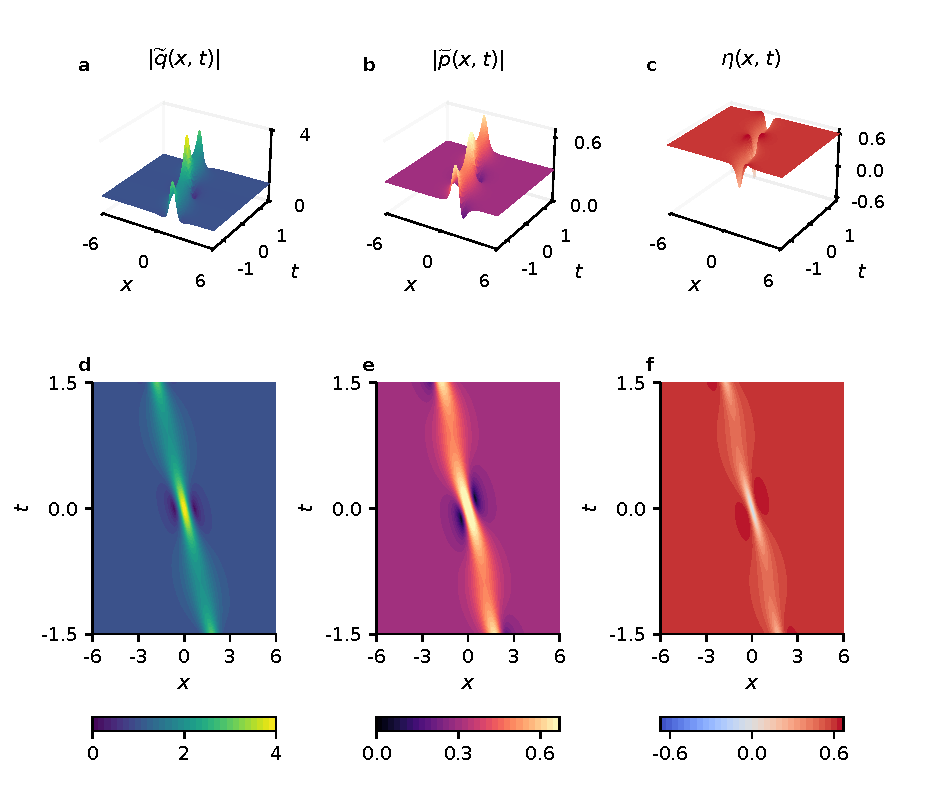
\includegraphics[width=\textwidth]{figures/one-soliton-fields.pdf}
\caption{单轨道物理三场 $|\widetilde q|,|\widetilde p|,\eta$ 的曲面 (上排) 与等值图 (下排). 参数见 \eqref{eq:numerical-parameters}; $x\in\lbrack-6,6\rbrack$, $t\in\lbrack-1.5,1.5\rbrack$.}
\label{fig:one}
\end{figure}

\FloatBarrier
\subsection{传播速度与内部振荡}
将背景传播因子分解为
\begin{align}
A_b=\operatorname{Re}F(\ii b)
&=-4\beta b^2-2\beta q_0^2-\dfrac{\eta_0}{a^2+b^2},\label{eq:velocity}\\
B_b=\operatorname{Im}F(\ii b)
&=-\alpha b-\dfrac{\eta_0b}{a(a^2+b^2)}.\label{eq:frequency}
\end{align}
\paragraph{传播函数实部和虚部的全部计算.}
从式 \eqref{eq:F} 原封不动代入 $k=\ii b$:
\begin{align*}
F(\ii b)
&=4\beta(\ii b)^2-\alpha\ii b-2\beta q_0^2
+\dfrac{\eta_0}{a(\ii b-a)}\\
&=-4\beta b^2-\ii\alpha b-2\beta q_0^2
+\dfrac{\eta_0(-a-\ii b)}{a(\ii b-a)(-a-\ii b)}.
\end{align*}
分母中
\[
(\ii b-a)(-a-\ii b)
=-\ii ab+b^2+a^2+\ii ab=a^2+b^2.
\]
所以有理项恰为
\[
\dfrac{\eta_0}{a(\ii b-a)}
=-\dfrac{\eta_0}{a^2+b^2}
-\ii\dfrac{\eta_0b}{a(a^2+b^2)}.
\]
其余各项的实虚性都已显现. 把没有 $\ii$ 的项与含 $\ii$ 的项分别合并, 就得到式 \eqref{eq:velocity}--\eqref{eq:frequency}. 因为所有参数为实数, 这里无需再对任何系数取实部或虚部. 同时
\[
F(-\ii b)=A_b-\ii B_b=\conj{F(\ii b)},
\]
与第8节使用的两个 $D_+$ 点的指数关系一致.

于是 $s=\kappa X-\ii\kappa B_bt$, 其中 $X=x-A_bt$. 显式矩阵 $P$ 关于 $x,t$ 的依赖由
\[
T=e^{2s}=e^{2\kappa X}e^{-2\ii\kappa B_bt}
\]
确定. 固定 $X$ 时, 若 $B_b\ne0$, 去相位三场具有周期
\begin{equation}\label{eq:internal-period}
T_t=\dfrac{\pi}{\kappa|B_b|}.
\end{equation}
\paragraph{包络移动和内部振荡怎样从同一个指数读出.}
不另设坐标, 先直接在原变量中展开:
\begin{align*}
s&=\kappa\{x-(A_b+\ii B_b)t\}
=\kappa(x-A_bt)-\ii\kappa B_bt,\\
2s&=2\kappa(x-A_bt)-2\ii\kappa B_bt,\\
|T|&=\left|e^{2\kappa(x-A_bt)}e^{-2\ii\kappa B_bt}\right|
=e^{2\kappa(x-A_bt)}.
\end{align*}
原文的 $X=x-A_bt$ 仅把已经出现的表达式命名, 本册没有额外变换. 要使 $|T|$ 保持相同, 就要保持 $x-A_bt$ 相同, 因而中心线是 $x=A_bt$. 同时比较 $t$ 与 $t+T_t$ 且沿这条同速轨迹移动 $x$, 有
\begin{align*}
T(x+A_bT_t,t+T_t)
&=e^{2\kappa[x+A_bT_t-A_b(t+T_t)]}
e^{-2\ii\kappa B_b(t+T_t)}\\
&=T(x,t)e^{-2\ii\kappa B_bT_t}.
\end{align*}
要让这个额外因子等于1, 其指数的相位必须是 $2\pi$ 的整数倍. 取正的完整相位周期,
\[
2\kappa|B_b|T_t=2\pi
\quad\Longrightarrow\quad
T_t=\dfrac{\pi}{\kappa|B_b|}.
\]
$P$ 是 $T,\conj{T}$ 的有理函数, $N(a)$ 是 $P$ 的矩阵多项式, 所以它们及规范三场都在这个平移后恢复原值. 这里的 $T_t$ 是原文给周期起的名称, 不是偏导数 $\partial_tT$. 本段证明了该值是一个周期, 不需要另行断言所有特殊参数下都没有更小周期.

若 $\alpha=-\dfrac{\eta_0}{a(a^2+b^2)}$, 则 $B_b=0$, 去相位三场仅依赖 $X$. 原场的模 $|\widetilde q|,|\widetilde p|$ 和反转 $\eta$ 也具有周期 \eqref{eq:internal-period}; 复场 $\widetilde q,\widetilde p$ 具有同一随动周期当且仅当 $\Omega T_t\in2\pi\mathbb Z$.

\paragraph{消除内部振荡与恢复共同相位.}
由 $b>q_0>0$ 可除以 $b$. 将 $B_b$ 的表达式设为零, 逐步得到
\begin{align*}
0&=-\alpha b-\dfrac{\eta_0b}{a(a^2+b^2)},\\
0&=-\alpha-\dfrac{\eta_0}{a(a^2+b^2)},\\
\alpha&=-\dfrac{\eta_0}{a(a^2+b^2)}.
\end{align*}
此时 $s$ 没有随 $t$ 单独变化的虚部, 所有规范场仅通过 $x-A_bt$ 变化. 这里不能把含 $|B_b|$ 的周期公式代入零分母; 正确结论是内部振荡消失.

当 $B_b\ne0$ 时, 规范场在一次随动周期后恢复, 原复光场还多出
\[
\dfrac{e^{-\ii\Omega(t+T_t)}}{e^{-\ii\Omega t}}
=e^{-\ii\Omega T_t}.
\]
由于 $q$ 有非零端态 $q_0$, 若要求整个复光场在同一次平移后恢复, 该因子必须为1. 这等价于 $\Omega T_t\in2\pi\mathbb Z$. 极化同理. 模长则不受这个因子影响, 反转本来就没有共同相位.

由 $P^2=P=P^\dagger$ 和 $\tr P=1$, 有 $|P_{12}|^2=P_{11}(1-P_{11})\le\dfrac{1}{4}$. 因而
\begin{equation}\label{eq:amplitude-bound}
|\widetilde q(x,t)|\le q_0+2b,\qquad |\widetilde q(0,0)|=q_0+2b.
\end{equation}
后一等式使用 $T(0,0)=1$ 和 $P_{12}(0,0)=\dfrac{1}{2}$. $P$ 在 $X\to\pm\infty$ 时趋于端态投影, 修正项为 $O(e^{-2\kappa|X|})$, 所以局域化尺度由 $\kappa$ 决定.

\paragraph{振幅估计每一步的不等式.}
Hermitian 性给出 $P_{21}=\conj{P_{12}}$. 取 $P^2=P$ 的第1行第1列:
\begin{align*}
P_{11}^2+P_{12}P_{21}&=P_{11},\\
|P_{12}|^2&=P_{11}-P_{11}^2
=\dfrac{1}{4}-\left(P_{11}-\dfrac{1}{2}\right)^2\le\dfrac{1}{4}.
\end{align*}
$P_{11}$ 为实数, 所以平方项非负, 从而 $|P_{12}|\le\dfrac{1}{2}$. 取式 \eqref{eq:finalfields} 中光场的模并应用三角不等式,
\begin{align*}
|\widetilde q|
&=\left|e^{-\ii\Omega t}(-q_0-4bP_{12})\right|
=|-q_0-4bP_{12}|\\
&\le q_0+4b|P_{12}|
\le q_0+2b.
\end{align*}
在 $x=t=0$ 时, 原文 $s=0$, $T=1$. 由 $\Delta_-=|T-h_0|^2+|1-h_0T|^2$,
\[
\Delta_-(0,0)=2(1-h_0)^2,
\qquad
P_{12}(0,0)=\dfrac{(1-h_0)(1-h_0)}{2(1-h_0)^2}=\dfrac{1}{2}.
\]
于是 $\widetilde q(0,0)=-q_0-2b$ 是负实数, 它的模正好达到上界. 本例等于 $1+2\cdot1.5=4$.

\paragraph{在原点同时检查两个介质分量.}
原点 $P$ 的四个元均为 $\dfrac{1}{2}$, 故式 \eqref{eq:Nfactor} 中的 $N(a)$ 在这里为
\[
N(a)=aI+\ii b(I-2P)
=\begin{pmatrix}a&-\ii b\\-\ii b&a\end{pmatrix}.
\]
将这四个元代入式 \eqref{eq:etacomponent}--\eqref{eq:pcomponent}:
\begin{align*}
\eta(0,0)
&=\dfrac{\eta_0}{a^2+b^2}
\left[a^2-b^2+\dfrac{\ii q_0}{a}
\{a(\ii b)-(-\ii b)a\}\right]\\
&=\dfrac{\eta_0}{a^2+b^2}(a^2-b^2-2bq_0),\\
\widetilde p(0,0)
&=\dfrac{\eta_0}{a^2+b^2}
\left[a(\ii b)-(-\ii b)a
+\dfrac{\ii q_0}{a}\{a^2-(-\ii b)(\ii b)\}\right]\\
&=\dfrac{\ii\eta_0}{a^2+b^2}
\left[2ab+\dfrac{q_0}{a}(a^2-b^2)\right].
\end{align*}
本例 $a^2+b^2=4+2.25=6.25$, 故
\begin{align*}
\eta(0,0)&=\dfrac{0.6}{6.25}(4-2.25-3)=-0.12,\\
\widetilde p(0,0)&=\dfrac{0.6\ii}{6.25}
\left[6+\dfrac{4-2.25}{2}\right]=0.66\ii,\\
|\widetilde p(0,0)|^2+\eta(0,0)^2
&=0.66^2+(-0.12)^2=0.4356+0.0144=0.45.
\end{align*}
因此图中中心处的介质偏离背景, 但仍严格位于同一个 Bloch 长度约束上.

\paragraph{指数衰减的量级为何是这个指数.}
由原文的 $P$ 公式, 当 $|T|\to0$ 时, 分子和分母都可以按 $T,\conj{T}$ 展开. 分母常数项是 $1+h_0^2>0$, 所以 $P-P_-$ 的每个元都是 $O(|T|)$. 当 $|T|\to\infty$ 时, 把分子分母同时除以 $|T|^2$, 常数主项给出 $P_+$, 其余是 $O(|T|^{-1})$. 又
\[
|T|=e^{2\kappa X},\qquad
|T|^{-1}=e^{-2\kappa X}.
\]
所以 $X\to-\infty$ 与 $X\to+\infty$ 的误差统一是 $O(e^{-2\kappa|X|})$. 光场是 $P$ 的线性表达式, 介质是 $P$ 的光滑有理矩阵表达式且分母 $a^2+b^2>0$, 因此三场保持同样的衰减量级.

参数 \eqref{eq:numerical-parameters} 给出 $A_b=-1.196$、$B_b=-1.572$ 和 $T_t\approx1.78748466439$. 图 \ref{fig:dynamics} 左图比较 $t=0,\dfrac{T_t}{4},\dfrac{T_t}{2}$ 时的随动截面; 右图比较 $\alpha=-0.048,0.5,1$ 时的中心光场模. 后两者的周期分别约为 $3.41840132897$ 和 $1.78748466439$, 而 $\alpha=-0.048$ 对应行波.
\paragraph{这些小数怎样算出.}
本例公共分母为 $a^2+b^2=6.25$. 逐项代入得
\begin{align*}
A_b&=-4\cdot0.1\cdot1.5^2-2\cdot0.1\cdot1^2-\dfrac{0.6}{6.25}\\
&=-0.9-0.2-0.096=-1.196,\\
B_b&=-1\cdot1.5-\dfrac{0.6\cdot1.5}{2\cdot6.25}
=-1.5-0.072=-1.572,\\
T_t&=\dfrac{\pi}{\dfrac{\sqrt{5}}{2}\cdot1.572}
\approx1.78748466439.
\end{align*}
当只把 $\alpha$ 改成 $0.5$ 时, $A_b$ 的表达式中没有 $\alpha$, 所以传播速度不变, 而
\[
B_b=-0.5\cdot1.5-0.072=-0.822,\qquad
T_t=\dfrac{\pi}{\dfrac{\sqrt{5}}{2}\cdot0.822}
\approx3.41840132897.
\]
当 $\alpha=-0.048$ 时,
\[
B_b=-(-0.048)\cdot1.5-0.072=0.072-0.072=0.
\]
同一个数也由临界参数式给出:
\[
-\dfrac{\eta_0}{a(a^2+b^2)}=-\dfrac{0.6}{2\cdot6.25}=-0.048.
\]
因此三条中心曲线的差别是内部振荡变化, 不是中心沿 $x$ 方向的移动速度变化. 图左在固定随动位置比较不同 $t$ 的截面, 正是为了能直接看见这个内部变化.
\begin{figure}[htbp]
\centering
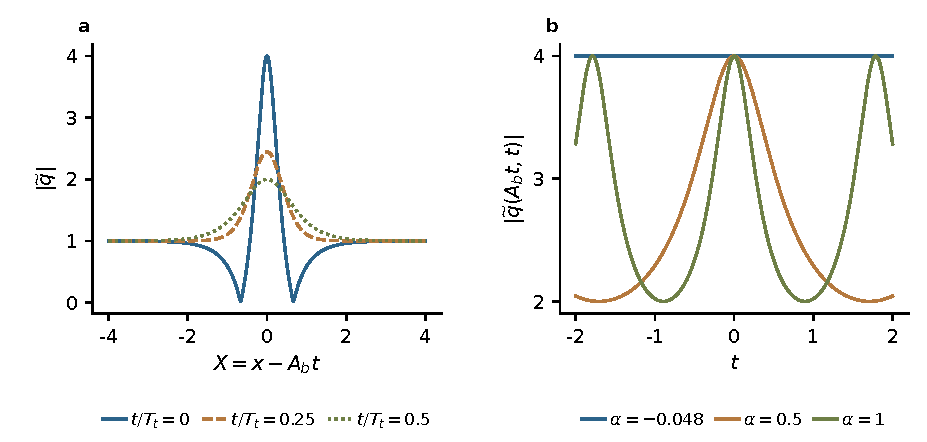
\includegraphics[width=\textwidth]{figures/one-soliton-dynamics.pdf}
\caption{单轨道光场的局域化与内部振荡. (a) 参数 \eqref{eq:numerical-parameters} 下的随动截面. (b) 改变 $\alpha$ 时 $|\widetilde q(A_bt,t)|$ 的变化, 其余参数固定.}
\label{fig:dynamics}
\end{figure}

\FloatBarrier
\subsection{参数影响与数值验证}
$\beta$ 改变式 \eqref{eq:velocity} 中的传播速度, 而不改变式 \eqref{eq:frequency} 中的内部频率. 图 \ref{fig:velocity} 取 $\beta=0,0.15$, 相应的 $A_b$ 为 $-0.096,-1.746$; 两者均有 $B_b=-1.572$ 和相同的随动周期. 虚线 $x=A_bt$ 表示中心轨迹.
\paragraph{分离两个参数作用的直接计算.}
在当前参数下, 速度对 $\beta$ 的依赖直接合并成
\[
A_b=-4\beta\cdot2.25-2\beta-0.096=-11\beta-0.096.
\]
代入图中两个取值得
\[
\beta=0:\quad A_b=-0.096,\qquad
\beta=0.15:\quad A_b=-11\cdot0.15-0.096=-1.746.
\]
两者都是负数, 所以 $t$ 增加时中心向更小的 $x$ 传播. 在固定 $q_0,a,\eta_0,b$ 下, 对原表达式求参数导数还可直接看出
\[
\dfrac{\partial A_b}{\partial\beta}=-4b^2-2q_0^2,\qquad
\dfrac{\partial B_b}{\partial\beta}=0,\qquad
\dfrac{\partial A_b}{\partial\alpha}=0,\qquad
\dfrac{\partial B_b}{\partial\alpha}=-b.
\]
因此在这个一轨道族中, 改变 $\beta$ 直接改变包络速度, 改变 $\alpha$ 直接改变内部振荡频率. 这几条参数偏导数只是原式的求导, 不需要额外的扰动理论. $\alpha$ 还通过 $\Omega$ 改变原复场的共同相位; 模长图没有显示这一相位变化.
\begin{figure}[htbp]
\centering
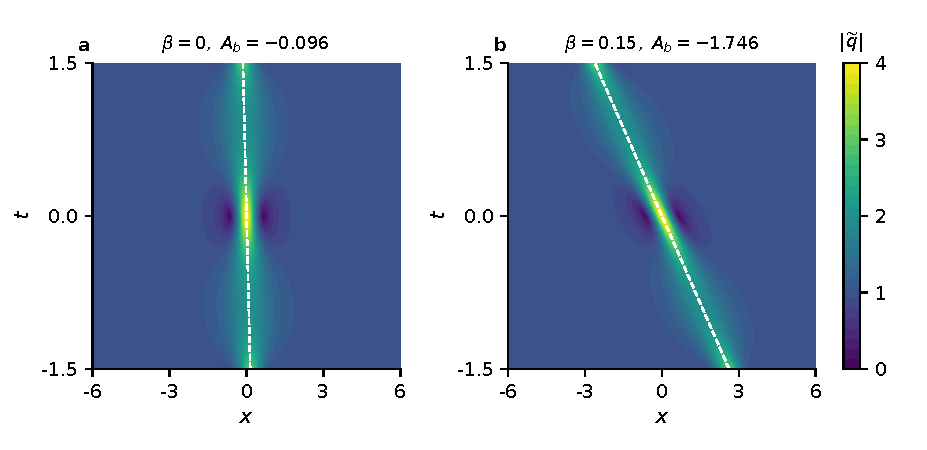
\includegraphics[width=\textwidth]{figures/one-soliton-velocity.pdf}
\caption{改变 $\beta$ 时的光场传播速度. 两图分别取 $\beta=0,0.15$, 其余参数同 \eqref{eq:numerical-parameters}; 白色虚线为 $x=A_bt$.}
\label{fig:velocity}
\end{figure}

对参数 \eqref{eq:numerical-parameters}, 采用 70 位十进制精度求解留数系统并对重构场求导, 得到表 \ref{tab:direct-residuals}. 导数由重构表达式直接计算. 双精度绘图实现与高精度实现的三个场在相同样点上的差均小于 $10^{-14}$; 等值图网格上的 Bloch 长度平方偏差及 $\eta$ 虚部均小于 $10^{-14}$. 两端 $x=\pm30$ 的三场误差均小于 $5.02\times10^{-29}$.
\begin{table}[htbp]
\centering
\caption{单轨道三场的高精度核验, 表内为样点最大绝对残差的向上舍入值}
\label{tab:direct-residuals}
\begin{tabular}{lc}
\toprule 检验对象 & 最大绝对误差\\\midrule
光场方程 & $1.87\times10^{-69}$\\
极化方程 & $8.26\times10^{-71}$\\
粒子数反转方程 & $1.50\times10^{-70}$\\
空间 Lax 方程 & $4.82\times10^{-70}$\\
时间 Lax 方程 & $1.95\times10^{-69}$\\
两共振原像的介质重构 & $1.12\times10^{-71}$\\
Bloch 长度平方 & $4.77\times10^{-72}$\\
\bottomrule
\end{tabular}
\end{table}

\paragraph{表中各行的残差究竟怎样形成.}
先在一个给定样点计算场及其所需导数, 再把方程的全部项移到左边. 表中前三行对应以下三个复数或实数的绝对值:
\begin{align*}
\left|\widetilde q_t
-\ii\alpha\left(\dfrac{\widetilde q_{xx}}{2}+|\widetilde q|^2\widetilde q\right)
-\beta(\widetilde q_{xxx}+6|\widetilde q|^2\widetilde q_x)-2\widetilde p\right|,\\
\left|\widetilde p_x-2\eta\widetilde q+2\ii a\widetilde p\right|,\\
\left|\eta_x+\conj{\widetilde q}\widetilde p+\widetilde q\conj{\widetilde p}\right|.
\end{align*}
例如, 第二条的加号来自把原方程右端的 $-2\ii a\widetilde p$ 移到左边. 它不是把原方程改成了另一个符号约定. 对每个样点各算一次, 再对所有样点取最大值, 得到表中的最大绝对残差. 在精确算术下这三项都为零; 高精度计算中的小非零值来自有限精度求值和求导.

\paragraph{原场导数与规范场导数的关系.}
共同相位只依赖 $t$, 所以所有 $x$ 导数都可以把它提出. 按原文的光场和介质重构式,
\begin{align*}
\widetilde q_x&=-4b e^{-\ii\Omega t}\partial_xP_{12},\\
\widetilde q_{xx}&=-4b e^{-\ii\Omega t}\partial_x^2P_{12},\\
\widetilde q_{xxx}&=-4b e^{-\ii\Omega t}\partial_x^3P_{12},\\
\widetilde q_t
&=e^{-\ii\Omega t}\left[\ii\Omega(q_0+4bP_{12})-4b\partial_tP_{12}\right],\\
\widetilde p_x&=-e^{-\ii\Omega t}\partial_xR_{12},\qquad
\eta_x=\partial_xR_{11}.
\end{align*}
时间导数中必须保留 $\ii\Omega(q_0+4bP_{12})$; 漏掉它就会把原方程与规范后的方程混用. 原文已有指数的导数也可直接计算:
\begin{align*}
\partial_xT&=2\kappa T,&
\partial_x\conj{T}&=2\kappa\conj{T},\\
\partial_tT&=-2\kappa F(\ii b)T,&
\partial_t\conj{T}&=-2\kappa\conj{F(\ii b)}\conj{T}.
\end{align*}
在这组式子里使用 $\partial_tT$ 表示偏导, 避免与原文的周期名称 $T_t$ 混淆. 将这些导数用于 $P$ 的原有有理表达式, 就能以乘法法则和商法则生成场导数, 不必使用网格差分.
本节末尾的``投影矩阵与三场导数的逐项求值''继续写出这些商法则的三阶展开、全部投影元的一阶导数, 以及介质矩阵的逐元导数, 可按该顺序直接执行求值.

\paragraph{两条 Lax 残差的符号.}
由式 \eqref{eq:Mspace} 及 $\phi=Me^{\ii\theta\sg}$, 对修正矩阵计算的两条残差是
\[
M_x-UM-\ii\lambda M\sg,\qquad
M_t-VM+\ii\lambda F M\sg.
\]
空间式的右乘项是负号移到左边, 时间式则因 $\theta_t=\lambda F$ 带相反的符号. 对每个谱测试点先取每个矩阵元绝对值的最大值, 再跨样点取最大值, 即得到表中两条 Lax 行. 两共振原像的核验则分别用 $z_a^+$、$z_a^-$ 代入式 \eqref{eq:RfromM}, 取两个矩阵之差的最大元绝对值. Bloch 行直接计算
\[
\left||\widetilde p|^2+\eta^2-
\eta_0^2\left(1+\dfrac{q_0^2}{a^2}\right)\right|.
\]

\paragraph{误差量级与边界检查怎样解释.}
70位十进制精度是内部运算的精度设定, 不是说每个结果都有70位相对有效数字. 对接近零的残差, 表格报告的是绝对误差. ``向上舍入''表示显示值不低于本次样点计算的最大值. 原文表格保留底稿的数值; 本详细版的复核结果另存于工程的检查报告中, 不把一次重跑得到的末位变化写成新的解析结论.
其中三条 PDE、两条 Lax 方程、留数系统和两共振重构的本次高精度结果保存在
\texttt{calculations/direct-rhp-results.json}; 原点三场、传播参数及指数因子保存在
\texttt{calculations/expanded-numerics-check.json}. 原文所述完整绘图网格误差按底稿保留, 本次没有重新生成全部网格和图像.

本例 $\kappa=\dfrac{\sqrt{5}}{2}$, 所以固定 $t$ 时理论端态衰减含有因子 $e^{-\sqrt{5}|x|}$. 在 $|x|=30$ 时,
\[
e^{-2\kappa\cdot30}=e^{-30\sqrt{5}}\approx7.36\times10^{-30}.
\]
这只是指数部分的数量级, 还要乘上依赖固定 $t$ 和场分量的有限系数, 所以不能直接把它当作三场误差的共同上界. 实际边界检查分别计算
\[
|\widetilde q-q_0e^{-\ii\Omega t}|,\qquad
\left|\widetilde p+\dfrac{\ii\eta_0q_0}{a}e^{-\ii\Omega t}\right|,\qquad
|\eta-\eta_0|.
\]
解析证明说明对所有允许参数和全部实 $x,t$ 的结构结论, 数值检查则检验本次实现是否在具体样点上正确执行了公式. 两者在本节中的作用由此区分.

\subsubsection*{补充计算: 投影矩阵与三场导数的逐项求值}
这一段继续使用原文的 $T,h_0,\kappa,\Delta_-,P,N,n_{jk}$, 不为任何分子或分母另取名称. 求偏导时固定全部模型参数和离散谱参数. 下面所有式子都只含原文已经定义的量及它们的导数, 所以既可以手工依次计算, 也可以按所写顺序直接用于数值求值.

\paragraph{先展开模平方及其空间、时间导数.}
原有指数满足
\begin{align*}
\partial_xT&=2\kappa T,
&\partial_x\conj{T}&=2\kappa\conj{T},\\
\partial_tT&=-2\kappa F(\ii b)T,
&\partial_t\conj{T}&=-2\kappa\conj{F(\ii b)}\conj{T}.
\end{align*}
因此不能把 $|T|^2$ 当成常数, 而须按两个指数的乘积求导:
\begin{align*}
|T|^2&=T\conj{T},\\
\partial_x|T|^2
&=(2\kappa T)\conj{T}
+T(2\kappa\conj{T})=4\kappa|T|^2,\\
\partial_x^2|T|^2
&=4\kappa\partial_x|T|^2
=16\kappa^2|T|^2,\\
\partial_x^3|T|^2
&=16\kappa^2\partial_x|T|^2
=64\kappa^3|T|^2,\\
\partial_t|T|^2
&=-2\kappa F(\ii b)T\conj{T}
-2\kappa\conj{F(\ii b)}T\conj{T}\\
&=-2\kappa\bigl(F(\ii b)+\conj{F(\ii b)}\bigr)|T|^2.
\end{align*}
同样, 对两个一次指数分别有
\begin{align*}
\partial_x^2T&=4\kappa^2T,
&\partial_x^2\conj{T}&=4\kappa^2\conj{T},\\
\partial_x^3T&=8\kappa^3T,
&\partial_x^3\conj{T}&=8\kappa^3\conj{T}.
\end{align*}
模平方的空间导数系数是 $4\kappa$, 一次指数的系数则是 $2\kappa$, 后面出现的 $2,4,8$ 倍数正是由这一区别产生.

\paragraph{把原分母的所有所需导数写全.}
原分母不作换名, 直接展开为
\[
\Delta_-=(1+h_0^2)(1+|T|^2)-2h_0(T+\conj{T}).
\]
连续求三次 $x$ 导数, 得
\begin{align*}
\partial_x\Delta_-
&=(1+h_0^2)\partial_x|T|^2
-2h_0(\partial_xT+\partial_x\conj{T})\\
&=4\kappa(1+h_0^2)|T|^2
-4\kappa h_0(T+\conj{T}),\\
\partial_x^2\Delta_-
&=4\kappa(1+h_0^2)\partial_x|T|^2
-4\kappa h_0(\partial_xT+\partial_x\conj{T})\\
&=16\kappa^2(1+h_0^2)|T|^2
-8\kappa^2h_0(T+\conj{T}),\\
\partial_x^3\Delta_-
&=16\kappa^2(1+h_0^2)\partial_x|T|^2
-8\kappa^2h_0(\partial_xT+\partial_x\conj{T})\\
&=64\kappa^3(1+h_0^2)|T|^2
-16\kappa^3h_0(T+\conj{T}).
\end{align*}
时间导数则保留原有传播函数及其共轭:
\begin{align*}
\partial_t\Delta_-
&=(1+h_0^2)\partial_t|T|^2
-2h_0(\partial_tT+\partial_t\conj{T})\\
&=-2\kappa(1+h_0^2)
\bigl(F(\ii b)+\conj{F(\ii b)}\bigr)|T|^2\\
&\quad+4\kappa h_0
\bigl(F(\ii b)T+\conj{F(\ii b)}\conj{T}\bigr).
\end{align*}
这些式子都可以只用已知的 $T,\conj{T}$ 直接求值. 后面出现 $\partial_x\Delta_-$ 等记法时, 它们就是以上完全写出的表达式, 并不代表需要另外求解的未知量.

\paragraph{右上投影元的乘积恒等式及其各阶右端.}
从原投影公式开始,
\begin{align*}
\Delta_-P_{12}
&=(T-h_0)(1-h_0\conj{T})\\
&=T-h_0-h_0|T|^2+h_0^2\conj{T}.
\end{align*}
右端的一至三阶空间导数依次是
\begin{align*}
\partial_x\bigl[(T-h_0)(1-h_0\conj{T})\bigr]
&=2\kappa T-4\kappa h_0|T|^2
+2\kappa h_0^2\conj{T}\\
&=2\kappa\bigl(T+h_0^2\conj{T}-2h_0|T|^2\bigr),\\
\partial_x^2\bigl[(T-h_0)(1-h_0\conj{T})\bigr]
&=4\kappa^2T-16\kappa^2h_0|T|^2
+4\kappa^2h_0^2\conj{T}\\
&=4\kappa^2\bigl(T+h_0^2\conj{T}-4h_0|T|^2\bigr),\\
\partial_x^3\bigl[(T-h_0)(1-h_0\conj{T})\bigr]
&=8\kappa^3T-64\kappa^3h_0|T|^2
+8\kappa^3h_0^2\conj{T}\\
&=8\kappa^3\bigl(T+h_0^2\conj{T}-8h_0|T|^2\bigr).
\end{align*}
时间导数也从原乘积直接展开:
\begin{align*}
\partial_t\bigl[(T-h_0)(1-h_0\conj{T})\bigr]
&=(-2\kappa F(\ii b)T)(1-h_0\conj{T})\\
&\quad+(T-h_0)
\bigl(2\kappa h_0\conj{F(\ii b)}\conj{T}\bigr)\\
&=-2\kappa F(\ii b)T
+2\kappa h_0F(\ii b)|T|^2\\
&\quad+2\kappa h_0\conj{F(\ii b)}|T|^2
-2\kappa h_0^2\conj{F(\ii b)}\conj{T}\\
&=-2\kappa\left[
F(\ii b)T+h_0^2\conj{F(\ii b)}\conj{T}
-h_0\bigl(F(\ii b)+\conj{F(\ii b)}\bigr)|T|^2
\right].
\end{align*}

\paragraph{由乘积恒等式连续求导, 得到可依次执行的递推.}
对 $\Delta_-P_{12}$ 求一次导数时, 两个因子都要求导:
\[
\Delta_-\partial_xP_{12}
+(\partial_x\Delta_-)P_{12}
=2\kappa\bigl(T+h_0^2\conj{T}-2h_0|T|^2\bigr).
\]
再求一次导数, 有
\begin{align*}
\Delta_-\partial_x^2P_{12}
+2(\partial_x\Delta_-)\partial_xP_{12}
+(\partial_x^2\Delta_-)P_{12}
&=4\kappa^2
\bigl(T+h_0^2\conj{T}-4h_0|T|^2\bigr).
\end{align*}
这里两个相同的中间项分别来自对 $\Delta_-\partial_xP_{12}$ 和 $(\partial_x\Delta_-)P_{12}$ 求导. 第三次求导时,
\begin{align*}
\Delta_-\partial_x^3P_{12}
&+3(\partial_x\Delta_-)\partial_x^2P_{12}\\
&+3(\partial_x^2\Delta_-)\partial_xP_{12}
+(\partial_x^3\Delta_-)P_{12}\\
&=8\kappa^3
\bigl(T+h_0^2\conj{T}-8h_0|T|^2\bigr).
\end{align*}
因此实际求值时可以按以下顺序, 每次只使用前面已经算出的低阶导数:
\begin{align*}
\partial_xP_{12}
&=\dfrac{2\kappa(T+h_0^2\conj{T}-2h_0|T|^2)
-(\partial_x\Delta_-)P_{12}}{\Delta_-},\\
\partial_x^2P_{12}
&=\dfrac{4\kappa^2(T+h_0^2\conj{T}-4h_0|T|^2)}{\Delta_-}\\
&\quad-\dfrac{2(\partial_x\Delta_-)\partial_xP_{12}
+(\partial_x^2\Delta_-)P_{12}}{\Delta_-},\\
\partial_x^3P_{12}
&=\dfrac{8\kappa^3(T+h_0^2\conj{T}-8h_0|T|^2)}{\Delta_-}\\
&\quad-\dfrac{3(\partial_x\Delta_-)\partial_x^2P_{12}
+3(\partial_x^2\Delta_-)\partial_xP_{12}
+(\partial_x^3\Delta_-)P_{12}}{\Delta_-}.
\end{align*}
原文已经证明 $\Delta_->0$, 所以每一次除法在所有实 $x,t$ 上都有意义. 这个递推没有引入分子的新名字, 也不需要用相邻网格点近似导数.

\paragraph{把递推消去, 写成完全展开的商法则形式.}
先把原 $P_{12}$ 代入一次导数公式:
\begin{align*}
\partial_xP_{12}
&=\dfrac{2\kappa(T+h_0^2\conj{T}-2h_0|T|^2)}{\Delta_-}\\
&\quad-\dfrac{(T-h_0)(1-h_0\conj{T})\partial_x\Delta_-}{\Delta_-^2}.
\end{align*}
对这一行逐项再求导, 相同项合并后得到
\begin{align*}
\partial_x^2P_{12}
&=\dfrac{4\kappa^2(T+h_0^2\conj{T}-4h_0|T|^2)}{\Delta_-}\\
&\quad-\dfrac{4\kappa(T+h_0^2\conj{T}-2h_0|T|^2)
\partial_x\Delta_-}{\Delta_-^2}\\
&\quad-\dfrac{(T-h_0)(1-h_0\conj{T})
\partial_x^2\Delta_-}{\Delta_-^2}\\
&\quad+\dfrac{2(T-h_0)(1-h_0\conj{T})
(\partial_x\Delta_-)^2}{\Delta_-^3}.
\end{align*}
再对各项求导, 三阶结果为
\begin{align*}
\partial_x^3P_{12}
&=\dfrac{8\kappa^3(T+h_0^2\conj{T}-8h_0|T|^2)}{\Delta_-}\\
&\quad-\dfrac{12\kappa^2(T+h_0^2\conj{T}-4h_0|T|^2)
\partial_x\Delta_-}{\Delta_-^2}\\
&\quad-\dfrac{6\kappa(T+h_0^2\conj{T}-2h_0|T|^2)
\partial_x^2\Delta_-}{\Delta_-^2}\\
&\quad+\dfrac{12\kappa(T+h_0^2\conj{T}-2h_0|T|^2)
(\partial_x\Delta_-)^2}{\Delta_-^3}\\
&\quad-\dfrac{(T-h_0)(1-h_0\conj{T})
\partial_x^3\Delta_-}{\Delta_-^2}\\
&\quad+\dfrac{6(T-h_0)(1-h_0\conj{T})
(\partial_x\Delta_-)(\partial_x^2\Delta_-)}{\Delta_-^3}\\
&\quad-\dfrac{6(T-h_0)(1-h_0\conj{T})
(\partial_x\Delta_-)^3}{\Delta_-^4}.
\end{align*}
这两种写法完全等价: 递推形式依次利用低阶结果, 展开形式则只有 $T,\conj{T}$、原分母及其已写出的导数. 例如三阶式中的系数3, 来自第三次对乘积求导时导数分配到两个因子的三种位置; 展开后对应系数 $12\kappa^2$, $6\kappa$, $12\kappa$.

\paragraph{右上投影元的时间导数.}
对原乘积恒等式求 $t$ 导数, 先得到
\begin{align*}
\Delta_-\partial_tP_{12}
+(\partial_t\Delta_-)P_{12}
&=-2\kappa\left[
F(\ii b)T+h_0^2\conj{F(\ii b)}\conj{T}\right.\\
&\hspace{35mm}\left.
-h_0\bigl(F(\ii b)+\conj{F(\ii b)}\bigr)|T|^2
\right].
\end{align*}
移项并代回原 $P_{12}$, 就有
\begin{align*}
\partial_tP_{12}
&=-\dfrac{2\kappa}{\Delta_-}
\left[F(\ii b)T+h_0^2\conj{F(\ii b)}\conj{T}\right.\\
&\hspace{34mm}\left.
-h_0\bigl(F(\ii b)+\conj{F(\ii b)}\bigr)|T|^2\right]\\
&\quad-\dfrac{(T-h_0)(1-h_0\conj{T})
\partial_t\Delta_-}{\Delta_-^2}.
\end{align*}
原场所需导数于是全部可以直接算出:
\begin{align*}
\widetilde q_x
&=-4b e^{-\ii\Omega t}\partial_xP_{12},\\
\widetilde q_{xx}
&=-4b e^{-\ii\Omega t}\partial_x^2P_{12},\\
\widetilde q_{xxx}
&=-4b e^{-\ii\Omega t}\partial_x^3P_{12},\\
\widetilde q_t
&=e^{-\ii\Omega t}
\left[\ii\Omega(q_0+4bP_{12})-4b\partial_tP_{12}\right].
\end{align*}
这里时间导数中的共同相位项仍须保留; 以上投影导数本身不能替代它.

\paragraph{其余三个投影元的一阶空间导数.}
先把原分子逐个展开, 不给它们另起名字:
\begin{align*}
|T-h_0|^2&=|T|^2-h_0(T+\conj{T})+h_0^2,\\
(1-h_0T)(\conj{T}-h_0)
&=\conj{T}-h_0-h_0|T|^2+h_0^2T,\\
|1-h_0T|^2&=1-h_0(T+\conj{T})+h_0^2|T|^2.
\end{align*}
故它们的导数分别为
\begin{align*}
\partial_x|T-h_0|^2
&=4\kappa|T|^2-2\kappa h_0(T+\conj{T}),\\
\partial_x\bigl[(1-h_0T)(\conj{T}-h_0)\bigr]
&=2\kappa\bigl(\conj{T}+h_0^2T-2h_0|T|^2\bigr),\\
\partial_x|1-h_0T|^2
&=-2\kappa h_0(T+\conj{T})+4\kappa h_0^2|T|^2.
\end{align*}
逐个应用商法则, 得
\begin{align*}
\partial_xP_{11}
&=\dfrac{4\kappa|T|^2-2\kappa h_0(T+\conj{T})}{\Delta_-}
-\dfrac{|T-h_0|^2\partial_x\Delta_-}{\Delta_-^2},\\
\partial_xP_{21}
&=\dfrac{2\kappa(\conj{T}+h_0^2T-2h_0|T|^2)}{\Delta_-}\\
&\quad-\dfrac{(1-h_0T)(\conj{T}-h_0)
\partial_x\Delta_-}{\Delta_-^2},\\
\partial_xP_{22}
&=\dfrac{-2\kappa h_0(T+\conj{T})+4\kappa h_0^2|T|^2}{\Delta_-}
-\dfrac{|1-h_0T|^2\partial_x\Delta_-}{\Delta_-^2}.
\end{align*}
因为 $\Delta_-$ 是实函数, 可直接从这些表达式检查
\[
\partial_xP_{21}=\conj{\partial_xP_{12}},
\qquad
\partial_xP_{11}+\partial_xP_{22}=0.
\]
第二式也可以从 $P_{11}+P_{22}=1$ 求导得到, 因而是检查实际实现的一项独立恒等式.

\paragraph{其余三个投影元的一阶时间导数.}
同样先求原分子的导数:
\begin{align*}
\partial_t|T-h_0|^2
&=-2\kappa\bigl(F(\ii b)+\conj{F(\ii b)}\bigr)|T|^2\\
&\quad+2\kappa h_0
\bigl(F(\ii b)T+\conj{F(\ii b)}\conj{T}\bigr),\\
\partial_t\bigl[(1-h_0T)(\conj{T}-h_0)\bigr]
&=-2\kappa\left[
\conj{F(\ii b)}\conj{T}+h_0^2F(\ii b)T\right.\\
&\hspace{29mm}\left.
-h_0\bigl(F(\ii b)+\conj{F(\ii b)}\bigr)|T|^2\right],\\
\partial_t|1-h_0T|^2
&=2\kappa h_0
\bigl(F(\ii b)T+\conj{F(\ii b)}\conj{T}\bigr)\\
&\quad-2\kappa h_0^2
\bigl(F(\ii b)+\conj{F(\ii b)}\bigr)|T|^2.
\end{align*}
再除以原分母并减去分母求导项:
\begin{align*}
\partial_tP_{11}
&=-\dfrac{2\kappa(F(\ii b)+\conj{F(\ii b)})|T|^2}{\Delta_-}\\
&\quad+\dfrac{2\kappa h_0
(F(\ii b)T+\conj{F(\ii b)}\conj{T})}{\Delta_-}
-\dfrac{|T-h_0|^2\partial_t\Delta_-}{\Delta_-^2},\\
\partial_tP_{21}
&=-\dfrac{2\kappa}{\Delta_-}
\left[\conj{F(\ii b)}\conj{T}+h_0^2F(\ii b)T\right.\\
&\hspace{33mm}\left.
-h_0(F(\ii b)+\conj{F(\ii b)})|T|^2\right]\\
&\quad-\dfrac{(1-h_0T)(\conj{T}-h_0)
\partial_t\Delta_-}{\Delta_-^2},\\
\partial_tP_{22}
&=\dfrac{2\kappa h_0
(F(\ii b)T+\conj{F(\ii b)}\conj{T})}{\Delta_-}\\
&\quad-\dfrac{2\kappa h_0^2
(F(\ii b)+\conj{F(\ii b)})|T|^2}{\Delta_-}
-\dfrac{|1-h_0T|^2\partial_t\Delta_-}{\Delta_-^2}.
\end{align*}
它们满足 $\partial_tP_{21}=\conj{\partial_tP_{12}}$ 及 $\partial_tP_{11}+\partial_tP_{22}=0$. 因而需要时间 Lax 检查时, 原矩阵 $P$ 的全部一阶时间导数也已具备.

\paragraph{从投影导数逐元得到 $N(a)$ 的导数.}
原定义 $N(k)=(k+\ii b)I-2\ii bP$ 在 $k=a$ 时给出
\begin{align*}
n_{11}&=a+\ii b-2\ii bP_{11},
&n_{12}&=-2\ii bP_{12},\\
n_{21}&=-2\ii bP_{21},
&n_{22}&=a+\ii b-2\ii bP_{22}.
\end{align*}
因此逐元求导的结果为
\begin{align*}
\partial_xn_{11}&=-2\ii b\partial_xP_{11},
&\partial_xn_{12}&=-2\ii b\partial_xP_{12},\\
\partial_xn_{21}&=-2\ii b\partial_xP_{21},
&\partial_xn_{22}&=-2\ii b\partial_xP_{22}.
\end{align*}
将它们合为矩阵, 得
\[
\partial_xN(a)=-2\ii b\partial_xP.
\]
由于 $b$ 为实数且 $P^\dagger=P$, 求导与共轭转置交换, 所以
\begin{align*}
\partial_xN(a)^\dagger
&=(\partial_xN(a))^\dagger\\
&=(-2\ii b\partial_xP)^\dagger
=2\ii b\partial_xP.
\end{align*}
逐个标量共轭时, 同样应使用
\[
\conj{\partial_xn_{jk}}
=2\ii b\conj{\partial_xP_{jk}}.
\]
这里 $n_{jk}$ 是原论文已有的 $N(a)$ 元素, 没有引入一个新的场或新的系数矩阵.

\paragraph{介质矩阵求导时的两个乘积及非对角负号.}
原介质矩阵为
\[
R=\dfrac{HN(a)R_\infty N(a)^\dagger H^{-1}}{a^2+b^2},
\qquad H=\diag(\ii,-\ii).
\]
$H,R_\infty,a,b$ 对 $x$ 都是常数, 所以乘积法则严格给出
\[
R_x=\dfrac{H\left[
(\partial_xN(a))R_\infty N(a)^\dagger
+N(a)R_\infty(\partial_xN(a))^\dagger
\right]H^{-1}}{a^2+b^2}.
\]
这个式子包含两项, 分别来自左右两个 $N$ 因子, 不可以只对左边的因子求导. 在 $H$ 的对角共轭作用下, 对角元不变, 两个非对角元反号. 特别地,
\begin{align*}
(R_x)_{11}
&=\dfrac{\left[
(\partial_xN(a))R_\infty N(a)^\dagger
+N(a)R_\infty(\partial_xN(a))^\dagger
\right]_{11}}{a^2+b^2},\\
(R_x)_{12}
&=-\dfrac{\left[
(\partial_xN(a))R_\infty N(a)^\dagger
+N(a)R_\infty(\partial_xN(a))^\dagger
\right]_{12}}{a^2+b^2}.
\end{align*}
结合原物理场 $\widetilde p=-e^{-\ii\Omega t}R_{12}$, 这个非对角负号与恢复极化的负号相消:
\begin{align*}
\eta_x&=(R_x)_{11},\\
\widetilde p_x
&=\dfrac{e^{-\ii\Omega t}}{a^2+b^2}
\left[
(\partial_xN(a))R_\infty N(a)^\dagger
+N(a)R_\infty(\partial_xN(a))^\dagger
\right]_{12}.
\end{align*}
这解释了为什么以下极化导数公式整体带正号, 虽然 $R$ 的右上元在原定义中等于 $-p$.

\paragraph{反转导数按原 $n_{jk}$ 分量式完全展开.}
由式 \eqref{eq:etacomponent}, 对每个乘积的两个因子分别求导, 得
\begin{align*}
\eta_x
&=\dfrac{\eta_0}{a^2+b^2}\left[
(\partial_xn_{11})\conj{n_{11}}
+n_{11}\conj{\partial_xn_{11}}\right.\\
&\quad-(\partial_xn_{12})\conj{n_{12}}
-n_{12}\conj{\partial_xn_{12}}\\
&\quad+\dfrac{\ii q_0}{a}\bigl(
(\partial_xn_{11})\conj{n_{12}}
+n_{11}\conj{\partial_xn_{12}}\\
&\hspace{32mm}\left.
-(\partial_xn_{12})\conj{n_{11}}
-n_{12}\conj{\partial_xn_{11}}\bigr)\right].
\end{align*}
再用已经得到的四个 $\partial_xn_{jk}$ 消去这些导数, 可以写成
\begin{align*}
\eta_x
&=\dfrac{2\ii b\eta_0}{a^2+b^2}\left[
-(\partial_xP_{11})\conj{n_{11}}
+n_{11}\conj{\partial_xP_{11}}\right.\\
&\quad+(\partial_xP_{12})\conj{n_{12}}
-n_{12}\conj{\partial_xP_{12}}\\
&\quad+\dfrac{\ii q_0}{a}\bigl(
-(\partial_xP_{11})\conj{n_{12}}
+n_{11}\conj{\partial_xP_{12}}\\
&\hspace{32mm}\left.
+(\partial_xP_{12})\conj{n_{11}}
-n_{12}\conj{\partial_xP_{11}}\bigr)\right].
\end{align*}
虽然这个写法显式含有 $\ii$, 整体仍为实数, 因为它与 Hermitian 矩阵 $R_x$ 的对角元相同. 实际计算中出现的极小虚部可以作为舍入误差的监测量, 不应先在代数推导中随意删去一项.

\paragraph{极化导数按原 $n_{jk}$ 分量式完全展开.}
由于 $e^{\ii\Omega t}$ 不依赖 $x$, 对式 \eqref{eq:pcomponent} 求导得到
\begin{align*}
\widetilde p_x
&=\dfrac{\eta_0e^{-\ii\Omega t}}{a^2+b^2}\left[
(\partial_xn_{11})\conj{n_{21}}
+n_{11}\conj{\partial_xn_{21}}\right.\\
&\quad-(\partial_xn_{12})\conj{n_{22}}
-n_{12}\conj{\partial_xn_{22}}\\
&\quad+\dfrac{\ii q_0}{a}\bigl(
(\partial_xn_{11})\conj{n_{22}}
+n_{11}\conj{\partial_xn_{22}}\\
&\hspace{32mm}\left.
-(\partial_xn_{12})\conj{n_{21}}
-n_{12}\conj{\partial_xn_{21}}\bigr)\right].
\end{align*}
继续代入 $\partial_xn_{jk}=-2\ii b\partial_xP_{jk}$, 得
\begin{align*}
\widetilde p_x
&=\dfrac{2\ii b\eta_0e^{-\ii\Omega t}}{a^2+b^2}\left[
-(\partial_xP_{11})\conj{n_{21}}
+n_{11}\conj{\partial_xP_{21}}\right.\\
&\quad+(\partial_xP_{12})\conj{n_{22}}
-n_{12}\conj{\partial_xP_{22}}\\
&\quad+\dfrac{\ii q_0}{a}\bigl(
-(\partial_xP_{11})\conj{n_{22}}
+n_{11}\conj{\partial_xP_{22}}\\
&\hspace{32mm}\left.
+(\partial_xP_{12})\conj{n_{21}}
-n_{12}\conj{\partial_xP_{21}}\bigr)\right].
\end{align*}
右端的每个投影导数都已经由前面的商法则明示. 因而检查介质 PDE 时, 可以先从显式场求导, 再与 $2\eta\widetilde q-2\ii a\widetilde p$ 及 $-(\conj{\widetilde q}\widetilde p+\widetilde q\conj{\widetilde p})$ 比较; 不必预先把待检查的 PDE 当作计算导数的公式.

\subsubsection*{补充计算: 投影端态误差的四个分量}
\paragraph{先以减去端态并通分的方式计算, 不只读出极限.}
原文给出的两个端态投影是
\[
P_- =\dfrac{1}{1+h_0^2}
\begin{pmatrix}h_0^2&-h_0\\-h_0&1\end{pmatrix},
\qquad
P_+ =\dfrac{1}{1+h_0^2}
\begin{pmatrix}1&-h_0\\-h_0&h_0^2\end{pmatrix}.
\]
例如在负端, 第1行第1列的差通分后为
\begin{align*}
P_{11}-(P_-)_{11}
&=\dfrac{|T-h_0|^2}{\Delta_-}-\dfrac{h_0^2}{1+h_0^2}\\
&=\dfrac{(1+h_0^2)|T-h_0|^2-h_0^2\Delta_-}
{(1+h_0^2)\Delta_-}.
\end{align*}
这个分子完全展开并抵消常数项, 得
\begin{align*}
&(1+h_0^2)\bigl[|T|^2-h_0(T+\conj{T})+h_0^2\bigr]\\
&\quad-h_0^2\bigl[(1+h_0^2)(1+|T|^2)-2h_0(T+\conj{T})\bigr]\\
&=(1-h_0^2)\bigl[(1+h_0^2)|T|^2-h_0(T+\conj{T})\bigr].
\end{align*}
非对角元的相同计算是
\begin{align*}
P_{12}-(P_-)_{12}
&=\dfrac{(T-h_0)(1-h_0\conj{T})}{\Delta_-}
+\dfrac{h_0}{1+h_0^2}\\
&=\dfrac{(1+h_0^2)(T-h_0-h_0|T|^2+h_0^2\conj{T})
+h_0\Delta_-}{(1+h_0^2)\Delta_-}\\
&=\dfrac{(1-h_0^2)(T-h_0^2\conj{T})}
{(1+h_0^2)\Delta_-}.
\end{align*}
因此负端的四个差值全部为
\begin{align*}
P_{11}-(P_-)_{11}
&=\dfrac{(1-h_0^2)
\bigl[T((1+h_0^2)\conj{T}-h_0)-h_0\conj{T}\bigr]}
{(1+h_0^2)\Delta_-},\\
P_{12}-(P_-)_{12}
&=\dfrac{(1-h_0^2)(T-h_0^2\conj{T})}
{(1+h_0^2)\Delta_-},\\
P_{21}-(P_-)_{21}
&=\dfrac{(1-h_0^2)(\conj{T}-h_0^2T)}
{(1+h_0^2)\Delta_-},\\
P_{22}-(P_-)_{22}
&=-\dfrac{(1-h_0^2)
\bigl[T((1+h_0^2)\conj{T}-h_0)-h_0\conj{T}\bigr]}
{(1+h_0^2)\Delta_-}.
\end{align*}
每个分子都明确带有 $T$ 或 $\conj{T}$ 因子. 在 $|T|\to0$ 时, 分母趋于 $(1+h_0^2)^2>0$, 所以四个差值逐个都是 $O(|T|)$.

\paragraph{正端也先给出精确差值.}
两个端态的非对角元相同, 故两条非对角差值与刚才完全一致. 对角元则得到
\begin{align*}
P_{11}-(P_+)_{11}
&=\dfrac{(1+h_0^2)|T-h_0|^2-\Delta_-}
{(1+h_0^2)\Delta_-}\\
&=\dfrac{(1-h_0^2)
\bigl[h_0(T+\conj{T})-(1+h_0^2)\bigr]}
{(1+h_0^2)\Delta_-},\\
P_{12}-(P_+)_{12}
&=\dfrac{(1-h_0^2)(T-h_0^2\conj{T})}
{(1+h_0^2)\Delta_-},\\
P_{21}-(P_+)_{21}
&=\dfrac{(1-h_0^2)(\conj{T}-h_0^2T)}
{(1+h_0^2)\Delta_-},\\
P_{22}-(P_+)_{22}
&=-\dfrac{(1-h_0^2)
\bigl[h_0(T+\conj{T})-(1+h_0^2)\bigr]}
{(1+h_0^2)\Delta_-}.
\end{align*}
在 $|T|\to\infty$ 时, 必须比较分子与分母的阶数, 不能看到分子也增长就断言误差不衰减. 先把原分母除以 $|T|^2$, 得
\[
\dfrac{\Delta_-}{|T|^2}
=(1+h_0^2)\left(1+\dfrac{1}{|T|^2}\right)
-2h_0\left(\dfrac{1}{T}+\dfrac{1}{\conj{T}}\right).
\]
其中用了 $\dfrac{T}{|T|^2}=\dfrac{1}{\conj{T}}$ 和 $\dfrac{\conj{T}}{|T|^2}=\dfrac{1}{T}$. 将四个差值的分子分母同时除以 $|T|^2$, 它们逐个变成
\begin{align*}
P_{11}-(P_+)_{11}
&=\dfrac{(1-h_0^2)
\left[h_0\left(\dfrac{1}{T}+\dfrac{1}{\conj{T}}\right)
-\dfrac{1+h_0^2}{|T|^2}\right]}
{(1+h_0^2)\dfrac{\Delta_-}{|T|^2}},\\
P_{12}-(P_+)_{12}
&=\dfrac{(1-h_0^2)
\left(\dfrac{1}{\conj{T}}-\dfrac{h_0^2}{T}\right)}
{(1+h_0^2)\dfrac{\Delta_-}{|T|^2}},\\
P_{21}-(P_+)_{21}
&=\dfrac{(1-h_0^2)
\left(\dfrac{1}{T}-\dfrac{h_0^2}{\conj{T}}\right)}
{(1+h_0^2)\dfrac{\Delta_-}{|T|^2}},\\
P_{22}-(P_+)_{22}
&=-\dfrac{(1-h_0^2)
\left[h_0\left(\dfrac{1}{T}+\dfrac{1}{\conj{T}}\right)
-\dfrac{1+h_0^2}{|T|^2}\right]}
{(1+h_0^2)\dfrac{\Delta_-}{|T|^2}}.
\end{align*}
现在分子明确含有 $1/T$, $1/\conj{T}$ 或 $1/|T|^2$, 分母趋于 $(1+h_0^2)^2>0$. 因而正端的四个差值逐个都是 $O(|T|^{-1})$. 这也是在较大 $|T|$ 处求值时可用的精确等价表达式, 可以避免先形成过大的共同因子再相除.

\paragraph{从投影误差具体传递到三个场.}
两端都有 $(P_\pm)_{12}=-h_0/(1+h_0^2)$, 而原恒等式 $2bh_0=q_0(1+h_0^2)$ 给出
\[
-q_0-4b(P_\pm)_{12}
=-q_0+\dfrac{4bh_0}{1+h_0^2}
=-q_0+2q_0=q_0.
\]
所以光场的端态差精确为
\[
\widetilde q-q_0e^{-\ii\Omega t}
=-4b e^{-\ii\Omega t}
\bigl(P_{12}-(P_\pm)_{12}\bigr).
\]
对介质使用原来的 $N_\pm=(a+\ii b)I-2\ii bP_\pm$, 有
\[
N(a)-N_\pm=-2\ii b(P-P_\pm).
\]
将两个乘积相减, 可以不遗漏任何交叉项地写成
\begin{align*}
&N(a)R_\infty N(a)^\dagger-N_\pm R_\infty N_\pm^\dagger\\
&\quad=(N(a)-N_\pm)R_\infty N(a)^\dagger
+N_\pm R_\infty(N(a)^\dagger-N_\pm^\dagger).
\end{align*}
右边展开后中间的 $-N_\pm R_\infty N(a)^\dagger$ 和 $+N_\pm R_\infty N(a)^\dagger$ 相消, 正好只留下左边的两项. 再使用前文已证明的端态介质等式, 就有
\begin{align*}
R-R_\infty
&=\dfrac{1}{a^2+b^2}H\Bigl[
(N(a)-N_\pm)R_\infty N(a)^\dagger\\
&\hspace{22mm}+N_\pm R_\infty(N(a)^\dagger-N_\pm^\dagger)
\Bigr]H^{-1}.
\end{align*}
再把 $N(a)-N_\pm=-2\ii b(P-P_\pm)$ 及其 Hermitian 共轭代入, 得到
\begin{align*}
R-R_\infty
&=-\dfrac{2\ii b}{a^2+b^2}H(P-P_\pm)R_\infty N(a)^\dagger H^{-1}\\
&\quad+\dfrac{2\ii b}{a^2+b^2}HN_\pm R_\infty(P-P_\pm)H^{-1}.
\end{align*}
因为 $P,P_\pm$ 是正交投影, 它们有界, 从而 $N(a),N_\pm$ 也有界. 上式的每个乘积都明确含有一个 $P-P_\pm$ 因子, 故介质误差与投影误差同阶. 最后由
\[
\widetilde p+\dfrac{\ii\eta_0q_0}{a}e^{-\ii\Omega t}
=-e^{-\ii\Omega t}(R_{12}-(R_\infty)_{12}),
\qquad
\eta-\eta_0=R_{11}-(R_\infty)_{11},
\]
得到两个物理介质分量的端态误差. 这就把 $O(|T|)$ 和 $O(|T|^{-1})$ 明确传递到三场. 用原有 $|T|=e^{2\kappa X}$, 负端为 $O(e^{2\kappa X})$, 正端为 $O(e^{-2\kappa X})$, 合起来是 $O(e^{-2\kappa|X|})$.

\paragraph{本例范数常数的根式化简.}
在 $q_0=1,b=1.5$ 的给定参数下,
\begin{align*}
h_0^2&=\left(\dfrac{3-\sqrt{5}}{2}\right)^2
=\dfrac{7-3\sqrt{5}}{2},\\
1+h_0^2&=\dfrac{9-3\sqrt{5}}{2}=3h_0,\\
c_1&=\dfrac{4\ii\kappa}{1+h_0^2}
=\dfrac{4\ii\sqrt{5}}{3(3-\sqrt{5})}\\
&=\dfrac{4\ii\sqrt{5}(3+\sqrt{5})}{3(9-5)}
=\dfrac{\ii(5+3\sqrt{5})}{3},\\
c_2&=-h_0^2c_1
=-\dfrac{4\ii\kappa h_0}{3}\\
&=-\dfrac{\ii\sqrt{5}(3-\sqrt{5})}{3}
=\dfrac{\ii(5-3\sqrt{5})}{3}.
\end{align*}
所以本例可直接使用
\[
c_1\approx3.902734644166456\ii,
\qquad
c_2\approx-0.569401310833123\ii.
\]
两者仍是原文的范数常数, 这些根式和小数只是把原式进一步算完, 不引入新的谱数据.


\subsection{数值计算的方法与结论范围}
数值图像由已证明的单轨道重构公式求值得到.
计算同时采用有限维留数系统与投影表达式, 用两种实现的相互比较核对代数重构.
三场方程、Lax 方程、Bloch 约束和两共振原像一致性的残差分别检验,
空间端态则在较大正负 $x$ 处核对.
这些样点检验与第 \ref{ch:verification} 节的解析证明相互配合:
解析证明建立全部实 $x,t$ 上的方程与边界, 数值结果展示局域结构及参数作用.

本文由此完成非零背景的直接散射、共振相容性、条件性 RHP 重构和指定单轨道的全局验证.
一般含反射数据的 RHP 可解性, 以及一般多轨道留数矩阵的全局非退化性,
需要进一步的分析, 不由本文的有限样点计算推出.
